% ============================================================
% PHARMACY V13
% MANAGEMENT INTELLIGENCE & DECISION-SUPPORT ARCHITECTURE
% Conceptual System Reference
% ============================================================
\documentclass[11pt,a4paper]{article}

\usepackage[a4paper,margin=24mm,headheight=14pt]{geometry}
\usepackage{fontspec}
\setmainfont{TeX Gyre Pagella}
\setsansfont{TeX Gyre Heros}
\usepackage{amsmath,amssymb}
\usepackage{booktabs,tabularx,longtable,array}
\usepackage{microtype}
\usepackage{enumitem}
\usepackage{xcolor}
\usepackage{tikz}
\usetikzlibrary{arrows.meta,positioning,fit,calc,shapes.geometric,backgrounds}
\usepackage{tcolorbox}
\tcbuselibrary{skins,breakable}
\usepackage{titlesec}
\usepackage{fancyhdr}
\usepackage{hyperref}
\usepackage{graphicx}

% ---------- Colors ----------
\definecolor{navy}{HTML}{17324D}
\definecolor{blue}{HTML}{245B8A}
\definecolor{teal}{HTML}{167C80}
\definecolor{green}{HTML}{3B7D4A}
\definecolor{gold}{HTML}{B27A16}
\definecolor{red}{HTML}{A5483D}
\definecolor{lightblue}{HTML}{EAF3F8}
\definecolor{lightteal}{HTML}{E9F6F4}
\definecolor{lightgold}{HTML}{FBF4E5}
\definecolor{lightred}{HTML}{F9ECEA}
\definecolor{lightgray}{HTML}{F3F5F7}
\definecolor{darkgray}{HTML}{424B53}

% ---------- Hyperref ----------
\hypersetup{
  colorlinks=true,
  linkcolor=navy,
  urlcolor=blue,
  citecolor=navy,
  pdftitle={Pharmacy V13 - Management Intelligence and Decision-Support Architecture},
  pdfauthor={Pharmacy V13},
  pdfsubject={Conceptual Management Intelligence Architecture}
}

% ---------- Page style ----------
\pagestyle{fancy}
\fancyhf{}
\lhead{\sffamily\small Pharmacy V13}
\rhead{\sffamily\small Management Intelligence Architecture}
\cfoot{\sffamily\small\thepage}
\renewcommand{\headrulewidth}{0.3pt}

\titleformat{\section}
  {\Large\bfseries\sffamily\color{navy}}
  {\thesection}{0.7em}{}
\titleformat{\subsection}
  {\large\bfseries\sffamily\color{blue}}
  {\thesubsection}{0.7em}{}

\setlist[itemize]{leftmargin=*,itemsep=3pt,topsep=4pt}
\setlist[enumerate]{leftmargin=*,itemsep=3pt,topsep=4pt}

% ---------- Boxes ----------
\newtcolorbox{principle}[1][]{
  enhanced,breakable,
  colback=lightblue,colframe=blue,
  boxrule=0.7pt,arc=2mm,
  title={#1},fonttitle=\bfseries\sffamily,
  left=5mm,right=5mm,top=3mm,bottom=3mm
}
\newtcolorbox{keyidea}[1][]{
  enhanced,breakable,
  colback=lightteal,colframe=teal,
  boxrule=0.7pt,arc=2mm,
  title={#1},fonttitle=\bfseries\sffamily,
  left=5mm,right=5mm,top=3mm,bottom=3mm
}
\newtcolorbox{warningbox}[1][]{
  enhanced,breakable,
  colback=lightgold,colframe=gold,
  boxrule=0.7pt,arc=2mm,
  title={#1},fonttitle=\bfseries\sffamily,
  left=5mm,right=5mm,top=3mm,bottom=3mm
}

% ---------- TikZ ----------
\tikzset{
  box/.style={
    rounded corners=2pt,draw=navy,fill=white,
    line width=.7pt,minimum height=10mm,
    text width=34mm,align=center,font=\sffamily\small
  },
  smallbox/.style={
    rounded corners=2pt,draw=blue,fill=lightblue,
    line width=.6pt,minimum height=9mm,
    text width=29mm,align=center,font=\sffamily\footnotesize
  },
  modelbox/.style={
    rounded corners=2pt,draw=teal,fill=lightteal,
    line width=.7pt,minimum height=10mm,
    text width=31mm,align=center,font=\sffamily\small
  },
  levelbox/.style={
    rounded corners=2pt,draw=navy,fill=white,
    line width=.8pt,minimum height=13mm,
    text width=39mm,align=center,font=\sffamily\small
  },
  arrow/.style={-{Latex[length=3mm]},draw=navy,line width=.8pt},
  feedback/.style={-{Latex[length=3mm]},draw=teal,line width=.9pt}
}

% ============================================================
\begin{document}

% ---------- Cover ----------
\begin{titlepage}
\thispagestyle{empty}
\vspace*{18mm}

\begin{center}
{\sffamily\color{navy}\fontsize{31}{36}\selectfont\bfseries PHARMACY V13\par}
\vspace{5mm}
{\sffamily\color{blue}\fontsize{20}{25}\selectfont
Management Intelligence\\
\& Decision-Support Architecture\par}

\vspace{12mm}
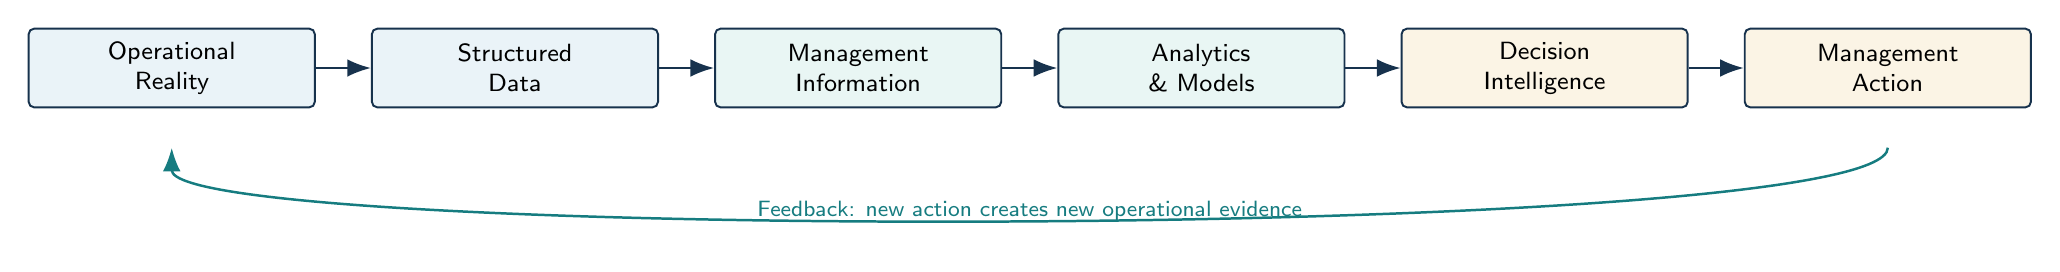
\begin{tikzpicture}[node distance=7mm]
\node[box,fill=lightblue] (o) {Operational\\Reality};
\node[box,fill=lightblue,right=of o] (d) {Structured\\Data};
\node[box,fill=lightteal,right=of d] (i) {Management\\Information};
\node[box,fill=lightteal,right=of i] (a) {Analytics\\\& Models};
\node[box,fill=lightgold,right=of a] (x) {Decision\\Intelligence};
\node[box,fill=lightgold,right=of x] (m) {Management\\Action};
\draw[arrow] (o)--(d);
\draw[arrow] (d)--(i);
\draw[arrow] (i)--(a);
\draw[arrow] (a)--(x);
\draw[arrow] (x)--(m);
\draw[feedback] ($(m.south)+(0,-5mm)$) .. controls +(0,-12mm) and +(0,-12mm) .. ($(o.south)+(0,-5mm)$);
\node[font=\sffamily\footnotesize\color{teal}] at ($(m.south)!0.5!(o.south)+(0,-13mm)$)
{Feedback: new action creates new operational evidence};
\end{tikzpicture}

\vfill

{\sffamily\large\color{darkgray}
\textit{From operational evidence to management intelligence}}
\vspace{8mm}

{\sffamily\large\bfseries Conceptual System Reference}\\[3mm]
{\sffamily 2026 \quad | \quad Version 1.0}

\vfill

\begin{minipage}{0.84\textwidth}
\centering
\small
This reference describes the conceptual architecture of Pharmacy V13 as an
integrated management intelligence and decision-support system. It focuses on
how the system observes pharmacy operations, transforms evidence into
information, applies analytical models, integrates AI-assisted reasoning, and
supports accountable management decisions.
\end{minipage}
\end{center}
\end{titlepage}

\tableofcontents
\newpage

% ============================================================
\section{Executive Concept}

Pharmacy V13 is best understood not as a collection of pharmacy records, but as
a \textbf{management intelligence system}. Its purpose is to transform the
continuous operational activity of a pharmacy into increasingly useful forms
of knowledge that support operational, tactical, and strategic management.

The central architecture is:

\begin{center}
\Large
\textbf{\color{navy}
Operational Reality $\rightarrow$ Data $\rightarrow$ Information
$\rightarrow$ Analysis $\rightarrow$ Intelligence $\rightarrow$ Decision
$\rightarrow$ Action $\rightarrow$ Feedback}
\end{center}

The database is therefore more than storage. It is the system's institutional
memory of operational events. The analytical layer transforms that memory into
evidence about demand, inventory, financial exposure, supplier behaviour,
expiry risk, and operational performance. The management interface brings
these signals together so that decision-makers can understand what is
happening, what may happen next, and where attention is required.

\begin{principle}[Core Management Principle]
\centering
\large
\textbf{V13 observes, measures, analyses, assesses risk, predicts, optimises,
supports decisions, and learns from the consequences of action.}
\end{principle}

The system is therefore designed as a \textbf{closed management loop}, not a
one-directional reporting pipeline.

% ============================================================
\section{Design Philosophy}

Five principles define the architecture.

\subsection{Evidence before interpretation}

Every analytical conclusion should ultimately be traceable to operational
evidence. Purchasing, stock movement, sales, inventory balances, expiry
information, and financial activity form the evidence foundation.

\subsection{Progressive transformation}

V13 progressively transforms information:

\[
\text{Event} \rightarrow
\text{Record} \rightarrow
\text{Indicator} \rightarrow
\text{Pattern} \rightarrow
\text{Risk} \rightarrow
\text{Prediction} \rightarrow
\text{Decision Support}.
\]

Each stage adds meaning without losing the relationship to the underlying
evidence.

\subsection{Question-driven analytics}

Analytical models exist because management has questions. A model should
therefore be introduced together with the decision question it helps answer.

\subsection{Integrated awareness}

Management should not have to inspect isolated reports and mentally assemble
the overall situation. V13 integrates multiple analytical signals into a
coherent management view.

\subsection{Human accountability}

AI and analytical models support management; they do not replace accountable
management judgement.

\begin{keyidea}[AI informs management; management decides.]
The architecture deliberately separates analytical intelligence from
institutional authority. A model may identify a risk, forecast a demand
pattern, or suggest a replenishment action, but the responsible manager remains
the decision-maker.
\end{keyidea}

% ============================================================
\section{Operational Evidence Layer}

The first layer represents the operational reality of the pharmacy.

\begin{center}
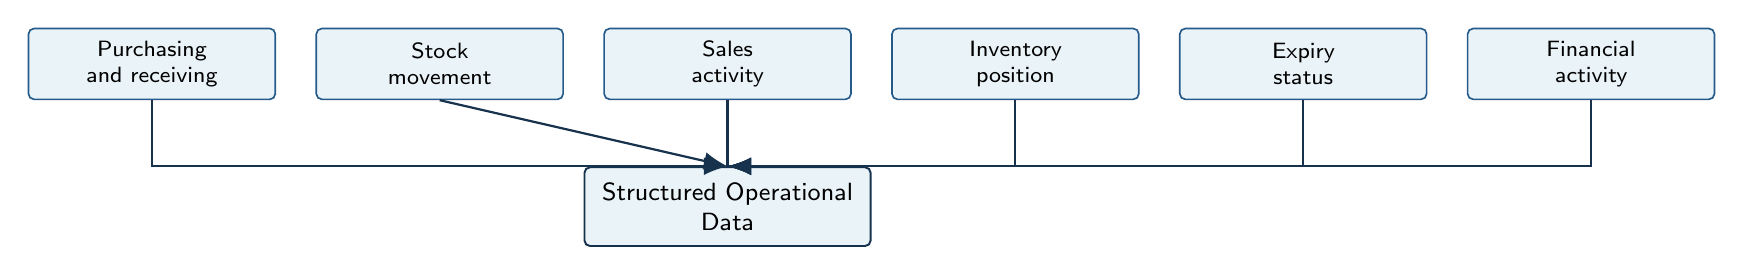
\begin{tikzpicture}[node distance=8mm and 5mm]
\node[smallbox] (p) {Purchasing\\and receiving};
\node[smallbox,right=of p] (s) {Stock\\movement};
\node[smallbox,right=of s] (sa) {Sales\\activity};
\node[smallbox,right=of sa] (in) {Inventory\\position};
\node[smallbox,right=of in] (ex) {Expiry\\status};
\node[smallbox,right=of ex] (fi) {Financial\\activity};

\node[box,below=13mm of $(s)!0.5!(in)$,fill=lightblue] (db)
{Structured Operational\\Data};

\draw[arrow] (p.south) |- (db.north);
\draw[arrow] (s.south) -- (db.north);
\draw[arrow] (sa.south) |- (db.north);
\draw[arrow] (in.south) |- (db.north);
\draw[arrow] (ex.south) |- (db.north);
\draw[arrow] (fi.south) |- (db.north);
\end{tikzpicture}
\end{center}

These domains answer different aspects of operational reality:

\begin{itemize}
\item \textbf{Purchasing} describes acquisition and supplier-related activity.
\item \textbf{Stock} describes quantities and movements through the system.
\item \textbf{Sales} describes observed demand and consumption behaviour.
\item \textbf{Inventory} describes the current and historical stock position.
\item \textbf{Expiry} describes time-related vulnerability of inventory.
\item \textbf{Financial activity} describes the monetary consequences of
      purchasing, sales, holding, and inventory decisions.
\end{itemize}

The important conceptual point is that these are not independent datasets.
Together they describe a connected operational system.

% ============================================================
\section{Data to Management Information}

Raw operational events become useful when they are structured and transformed
into management information.

\begin{center}
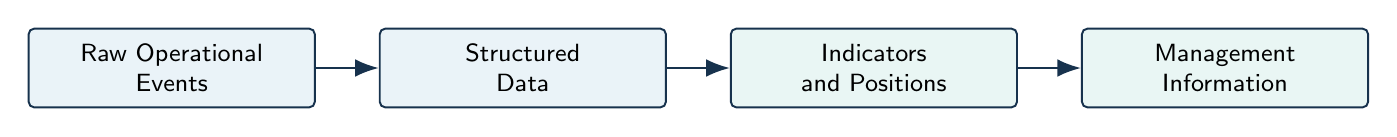
\begin{tikzpicture}[node distance=8mm]
\node[box,fill=lightblue] (raw) {Raw Operational\\Events};
\node[box,fill=lightblue,right=of raw] (structured) {Structured\\Data};
\node[box,fill=lightteal,right=of structured] (ind) {Indicators\\and Positions};
\node[box,fill=lightteal,right=of ind] (mi) {Management\\Information};

\draw[arrow] (raw)--(structured);
\draw[arrow] (structured)--(ind);
\draw[arrow] (ind)--(mi);
\end{tikzpicture}
\end{center}

\begin{center}
\renewcommand{\arraystretch}{1.35}
\begin{tabularx}{\textwidth}{>{\bfseries}p{31mm} X X}
\toprule
Operational domain & Management information & Management question \\
\midrule
Purchasing & Supplier activity, acquisition pattern, purchasing cost &
Are purchasing decisions aligned with demand and inventory requirements? \\
Sales & Demand pattern, consumption rate, variability &
What is being demanded, and how stable is that demand? \\
Stock & On-hand quantity, movement, stock coverage &
Where is inventory sufficient, constrained, or excessive? \\
Inventory & Value, composition, turnover, concentration &
Where is capital committed to inventory? \\
Expiry & Remaining shelf-life exposure, vulnerable quantities &
Where could stock become operationally or financially vulnerable? \\
Financial activity & Revenue, acquisition cost, inventory-related exposure &
What are the financial consequences of operational decisions? \\
\bottomrule
\end{tabularx}
\end{center}

Management information is therefore a structured interpretation of operational
evidence, not simply a more attractive database screen.

% ============================================================
\section{Information to Analytical Understanding}

Once management information exists, analytical models can identify patterns,
uncertainty, risks, and possible actions.

\begin{center}
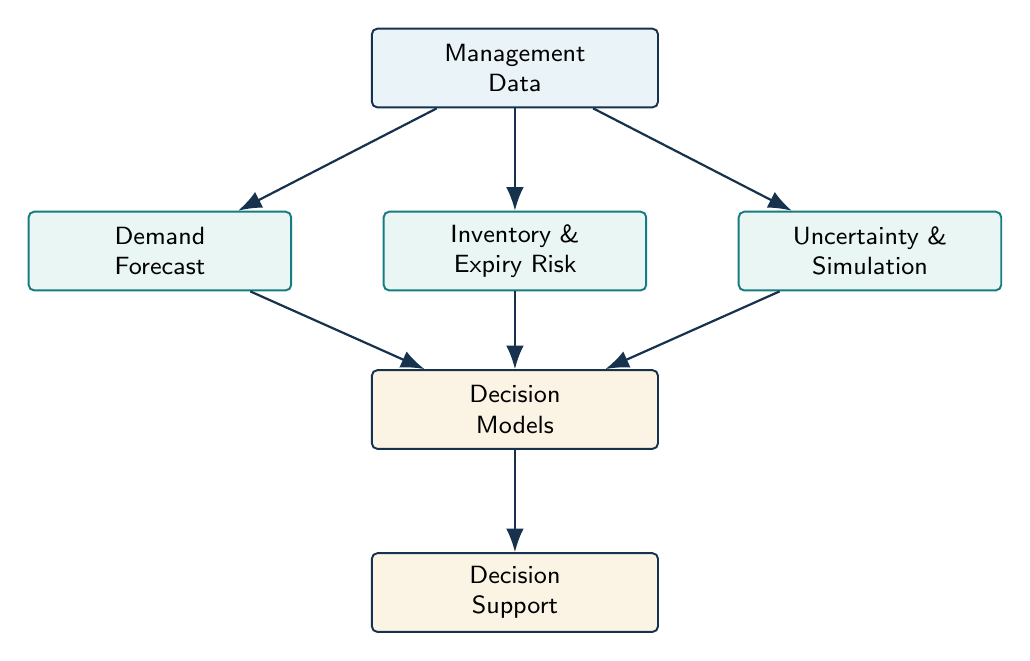
\begin{tikzpicture}[node distance=7mm and 8mm]
\node[box,fill=lightblue] (data) {Management\\Data};

\node[modelbox,below left=13mm and 10mm of data] (forecast)
{Demand\\Forecast};
\node[modelbox,below=13mm of data] (risk)
{Inventory \&\\Expiry Risk};
\node[modelbox,below right=13mm and 10mm of data] (sim)
{Uncertainty \&\\Simulation};

\node[box,below=15mm of $(forecast)!0.5!(sim)$,fill=lightgold] (decision)
{Decision\\Models};

\node[box,below=13mm of decision,fill=lightgold] (support)
{Decision\\Support};

\draw[arrow] (data)--(forecast);
\draw[arrow] (data)--(risk);
\draw[arrow] (data)--(sim);
\draw[arrow] (forecast)--(decision);
\draw[arrow] (risk)--(decision);
\draw[arrow] (sim)--(decision);
\draw[arrow] (decision)--(support);
\end{tikzpicture}
\end{center}

This creates four analytical levels.

\begin{description}
\item[\textbf{Descriptive}] What happened? What is happening now?
\item[\textbf{Diagnostic}] What patterns or relationships help explain the
current situation?
\item[\textbf{Predictive}] What is likely to happen next, and under what
uncertainty?
\item[\textbf{Prescriptive}] Given the evidence and constraints, what options
deserve management consideration?
\end{description}

% ============================================================
\section{Management Questions and Analytical Models}

The models in V13 should be understood through the questions they answer.

\begin{center}
\renewcommand{\arraystretch}{1.45}
\begin{tabularx}{\textwidth}{>{\bfseries}p{34mm} X X}
\toprule
Model & Primary management question & Decision-support role \\
\midrule
Forecasting & What demand should we expect? &
Estimate future demand from historical and contextual patterns. \\
Reorder Point & When should replenishment be triggered? &
Translate expected demand and lead time into an operational trigger. \\
Safety Stock & How much protection against uncertainty is needed? &
Protect service levels against demand and supply variability. \\
EOQ & What replenishment quantity balances relevant costs? &
Frame the trade-off between ordering and holding costs. \\
ABC Analysis & Which items deserve the greatest management attention? &
Prioritise managerial control according to value or importance. \\
Expiry Risk & Where could inventory become vulnerable because of time? &
Identify stock whose remaining life may not match expected consumption. \\
Monte Carlo & What could happen under uncertainty? &
Explore distributions of outcomes rather than relying only on point estimates. \\
AI Integrated View & What deserves attention now, and why? &
Synthesize multiple signals into an interpretable management view. \\
\bottomrule
\end{tabularx}
\end{center}

% ============================================================
\section{Demand Forecasting}

\subsection{Management question}

\begin{principle}[Question]
\centering
\Large \textbf{What demand should we expect over the next planning period?}
\end{principle}

Forecasting converts historical demand into an estimate of future demand.

A generic representation is:

\[
\widehat{D}_{t+h}
=
f(D_t,D_{t-1},\ldots,D_{t-k},X_t),
\]

where \(D\) represents observed demand and \(X\) represents relevant contextual
variables.

The exact forecasting method may vary with data volume, stability, seasonality,
and operational requirements. The architecture does not depend on one
particular forecasting algorithm.

\subsection{Management interpretation}

The forecast is not a statement of certainty. It is an evidence-based
expectation that should be accompanied, where appropriate, by uncertainty or
confidence information.

The management value is created when forecast information is connected to
inventory decisions:

\[
\text{Forecast}
\rightarrow
\text{Expected Consumption}
\rightarrow
\text{Stock Coverage}
\rightarrow
\text{Replenishment Decision}.
\]

% ============================================================
\section{Reorder Point and Safety Stock}

\subsection{Reorder Point}

\begin{principle}[Question]
\centering
\Large \textbf{When should replenishment be triggered?}
\end{principle}

A conceptual reorder-point model is:

\[
ROP = \mu_D L + SS,
\]

where

\begin{itemize}
\item \(\mu_D\) is expected demand per unit time,
\item \(L\) is replenishment lead time,
\item \(SS\) is safety stock.
\end{itemize}

The first term represents expected demand during lead time. Safety stock
provides additional protection against uncertainty.

\subsection{Safety Stock}

\begin{principle}[Question]
\centering
\Large \textbf{How much uncertainty protection is needed?}
\end{principle}

A simplified formulation is:

\[
SS=z\sigma_{DL},
\]

where \(z\) represents a chosen service-level factor and
\(\sigma_{DL}\) represents uncertainty in demand during lead time.

In real deployment, the uncertainty model should reflect the available
evidence and whether demand and lead-time variability are independent,
correlated, seasonal, or otherwise structured.

\begin{keyidea}[Operational meaning]
ROP answers \emph{when to review or trigger replenishment}; safety stock answers
\emph{how much uncertainty protection is carried around the expected
requirement}.
\end{keyidea}

% ============================================================
\section{Economic Order Quantity}

\subsection{Management question}

\begin{principle}[Question]
\centering
\Large \textbf{What order quantity balances ordering and holding costs?}
\end{principle}

The classical EOQ expression is:

\[
EOQ=\sqrt{\frac{2DS}{H}},
\]

where \(D\) is annual demand, \(S\) is ordering cost per order, and \(H\) is
annual holding cost per unit.

EOQ is a decision-support model, not an automatic purchasing instruction.

It provides a useful economic reference point for the relationship between:

\[
\text{Order frequency}
\quad\leftrightarrow\quad
\text{Order size}
\quad\leftrightarrow\quad
\text{Holding exposure}.
\]

The classical model assumes relatively stable demand and simplified cost
conditions. Real pharmacy decisions may also depend on shelf life, supplier
constraints, minimum order quantities, storage capacity, service requirements,
and regulatory or clinical considerations.

% ============================================================
\section{ABC Analysis}

\subsection{Management question}

\begin{principle}[Question]
\centering
\Large \textbf{Which inventory items deserve the greatest management attention?}
\end{principle}

A common starting measure is annual consumption value:

\[
ACV_i=D_i C_i,
\]

where \(D_i\) is annual demand for item \(i\) and \(C_i\) is its unit cost.

Items can then be ranked by \(ACV\), followed by cumulative analysis.

ABC analysis converts a large inventory population into management priorities.

\begin{center}
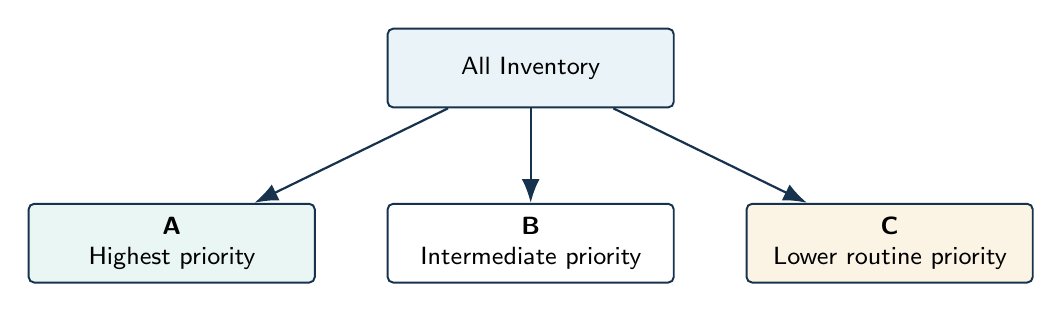
\begin{tikzpicture}[node distance=9mm]
\node[box,fill=lightblue] (all) {All Inventory};
\node[box,fill=lightteal,below left=12mm and 9mm of all] (a)
{\textbf{A}\\Highest priority};
\node[box,fill=white,below=12mm of all] (b)
{\textbf{B}\\Intermediate priority};
\node[box,fill=lightgold,below right=12mm and 9mm of all] (c)
{\textbf{C}\\Lower routine priority};
\draw[arrow] (all)--(a);
\draw[arrow] (all)--(b);
\draw[arrow] (all)--(c);
\end{tikzpicture}
\end{center}

The exact percentage thresholds are policy choices and should be documented
rather than treated as universal laws.

% ============================================================
\section{Expiry Risk}

\subsection{Management question}

\begin{principle}[Question]
\centering
\Large \textbf{Where could inventory become vulnerable because remaining
shelf life is shorter than expected consumption time?}
\end{principle}

A simple conceptual comparison is:

\[
\text{Days to Consume}
\approx
\frac{Q}{\widehat d},
\]

where \(Q\) is available quantity and \(\widehat d\) is expected daily demand.

This estimate can be compared with the remaining time to expiry \(T_e\).

The central relationship is:

\[
\text{Expected consumption time}
\quad\text{vs.}\quad
\text{remaining shelf life}.
\]

If expected consumption time approaches or exceeds remaining shelf life,
management attention should increase.

Expiry risk should not be reduced to a single binary flag. A useful management
assessment can consider:

\begin{itemize}
\item quantity at risk,
\item unit value and total financial exposure,
\item expected demand,
\item remaining shelf life,
\item demand variability,
\item replenishment commitments,
\item operational alternatives,
\item relevant pharmacy policies and regulations.
\end{itemize}

% ============================================================
\section{Monte Carlo Uncertainty Analysis}

\subsection{Management question}

\begin{principle}[Question]
\centering
\Large \textbf{What could happen when demand and supply conditions are uncertain?}
\end{principle}

Point estimates can hide uncertainty. Monte Carlo simulation addresses this by
repeatedly sampling plausible values from specified distributions.

For example, let simulated demand and lead time be:

\[
(D^{(1)},L^{(1)}),\ldots,(D^{(N)},L^{(N)}).
\]

For each simulation, the system can calculate a resulting inventory outcome.
The simulations collectively form a distribution of possible outcomes.

A conceptual stockout probability can be expressed as:

\[
P(\text{Stockout})
\approx
\frac{1}{N}
\sum_{j=1}^{N}
I\!\left(Q < D_{L}^{(j)}\right),
\]

where \(I(\cdot)\) is an indicator function and \(D_L^{(j)}\) is simulated
demand over simulated lead time.

\begin{center}
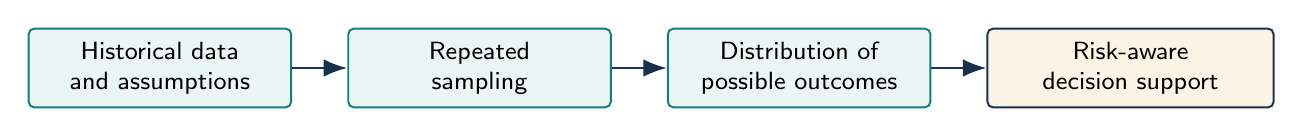
\begin{tikzpicture}[node distance=7mm]
\node[modelbox] (inputs) {Historical data\\and assumptions};
\node[modelbox,right=of inputs] (sample) {Repeated\\sampling};
\node[modelbox,right=of sample] (out) {Distribution of\\possible outcomes};
\node[box,fill=lightgold,right=of out] (decision) {Risk-aware\\decision support};
\draw[arrow] (inputs)--(sample);
\draw[arrow] (sample)--(out);
\draw[arrow] (out)--(decision);
\end{tikzpicture}
\end{center}

Monte Carlo therefore changes the management question from:

\begin{quote}
``What is the expected value?''
\end{quote}

to a richer question:

\begin{quote}
``What range of outcomes is plausible, how likely are adverse outcomes, and
what would their consequences be?''
\end{quote}

% ============================================================
\section{Integrated Decision-Support Architecture}

The strength of V13 emerges when individual models are not treated as isolated
reports.

\begin{center}
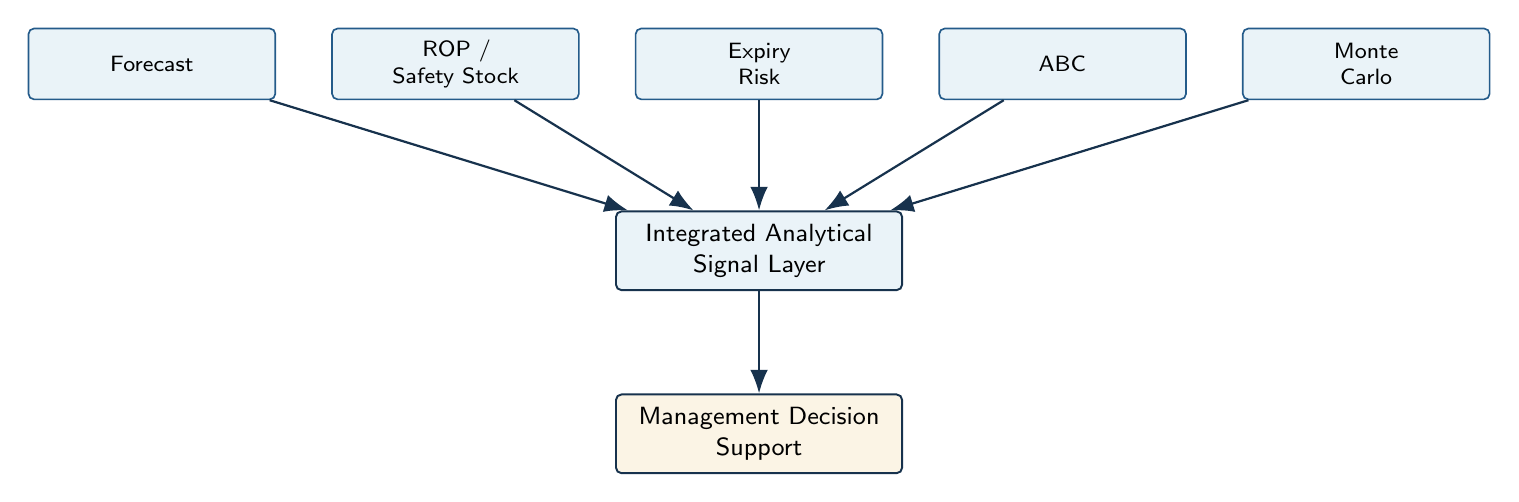
\begin{tikzpicture}[node distance=8mm and 7mm]
\node[smallbox] (f) {Forecast};
\node[smallbox,right=of f] (r) {ROP /\\Safety Stock};
\node[smallbox,right=of r] (e) {Expiry\\Risk};
\node[smallbox,right=of e] (a) {ABC};
\node[smallbox,right=of a] (m) {Monte\\Carlo};

\node[box,below=14mm of e,fill=lightblue] (integration)
{Integrated Analytical\\Signal Layer};

\node[box,below=13mm of integration,fill=lightgold]
(decision) {Management Decision\\Support};

\draw[arrow] (f)--(integration);
\draw[arrow] (r)--(integration);
\draw[arrow] (e)--(integration);
\draw[arrow] (a)--(integration);
\draw[arrow] (m)--(integration);
\draw[arrow] (integration)--(decision);
\end{tikzpicture}
\end{center}

The integrated layer can reveal relationships that individual models may not
show on their own.

For example:

\[
\text{High forecast}
+
\text{low stock}
+
\text{long lead time}
\Rightarrow
\text{high replenishment attention}.
\]

Or:

\[
\text{Low forecast}
+
\text{high stock}
+
\text{short remaining shelf life}
\Rightarrow
\text{high expiry exposure}.
\]

These are not automatic decisions. They are \textbf{management signals} that
combine evidence from several dimensions.

% ============================================================
\section{AI-Integrated Management View}

AI is most valuable in V13 when it sits above the analytical evidence rather
than replacing it.

\begin{center}
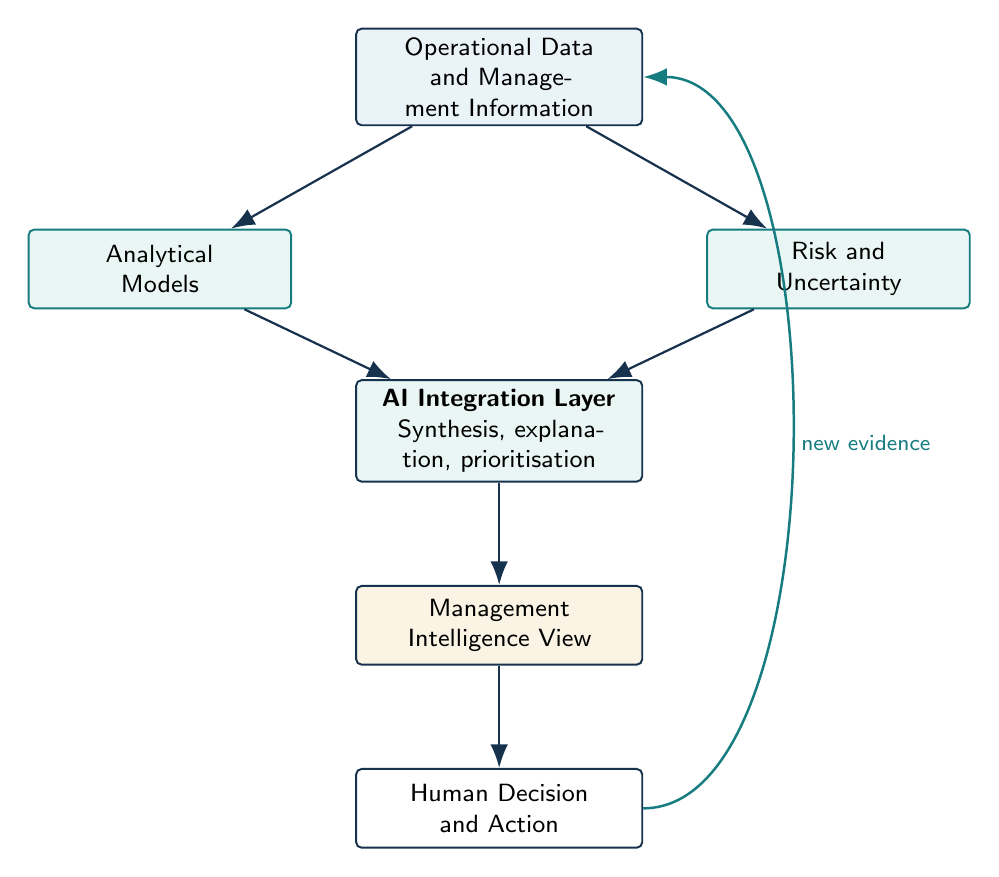
\begin{tikzpicture}[node distance=7mm and 9mm]
\node[box,fill=lightblue] (data)
{Operational Data\\and Management Information};

\node[modelbox,below left=13mm and 8mm of data] (analytics)
{Analytical\\Models};

\node[modelbox,below right=13mm and 8mm of data] (risk)
{Risk and\\Uncertainty};

\node[box,below=14mm of $(analytics)!0.5!(risk)$,fill=lightteal]
(ai)
{\textbf{AI Integration Layer}\\Synthesis, explanation, prioritisation};

\node[box,below=13mm of ai,fill=lightgold]
(cockpit)
{Management\\Intelligence View};

\node[box,below=13mm of cockpit]
(action)
{Human Decision\\and Action};

\draw[arrow] (data)--(analytics);
\draw[arrow] (data)--(risk);
\draw[arrow] (analytics)--(ai);
\draw[arrow] (risk)--(ai);
\draw[arrow] (ai)--(cockpit);
\draw[arrow] (cockpit)--(action);
\draw[feedback] (action.east) .. controls +(25mm,0) and +(25mm,0) ..
  node[right,font=\sffamily\footnotesize\color{teal}]
  {new evidence} (data.east);
\end{tikzpicture}
\end{center}

\subsection{What AI adds}

An AI-assisted management layer can help with:

\begin{itemize}
\item \textbf{Signal synthesis:} combine multiple analytical outputs.
\item \textbf{Prioritisation:} identify issues that deserve attention first.
\item \textbf{Explanation:} translate analytical outputs into understandable
      management language.
\item \textbf{Anomaly detection:} highlight unusual operational behaviour.
\item \textbf{Scenario comparison:} help managers compare possible actions.
\item \textbf{Natural-language interaction:} allow managers to ask questions
      about the evidence and analytical state.
\item \textbf{Decision narratives:} explain why an item or situation has been
      flagged and identify the evidence supporting the flag.
\end{itemize}

\subsection{AI evidence stack}

A trustworthy AI management response should conceptually draw from:

\[
\boxed{
\text{Data}
+
\text{Indicators}
+
\text{Models}
+
\text{Policies}
+
\text{Context}
\rightarrow
\text{Management Insight}
}
\]

The AI layer should preserve source traceability, expose uncertainty where
appropriate, and distinguish evidence from inference.

\begin{warningbox}[AI Governance Boundary]
AI should not silently convert a statistical prediction into a factual claim,
or a recommendation into an authorised management action. Every important
recommendation should remain reviewable by the responsible decision-maker.
\end{warningbox}

% ============================================================
\section{Management Hierarchy}

V13 supports three complementary management levels.

\begin{center}
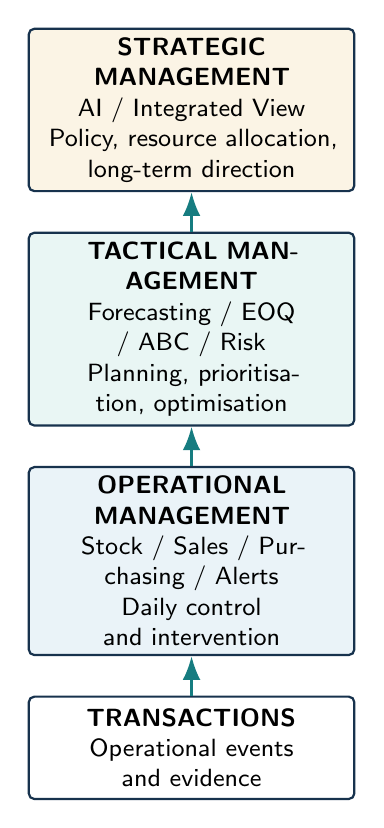
\begin{tikzpicture}[node distance=5mm]
\node[levelbox,fill=lightgold] (strategic)
{\textbf{STRATEGIC MANAGEMENT}\\
AI / Integrated View\\
Policy, resource allocation, long-term direction};

\node[levelbox,fill=lightteal,below=of strategic] (tactical)
{\textbf{TACTICAL MANAGEMENT}\\
Forecasting / EOQ / ABC / Risk\\
Planning, prioritisation, optimisation};

\node[levelbox,fill=lightblue,below=of tactical] (operational)
{\textbf{OPERATIONAL MANAGEMENT}\\
Stock / Sales / Purchasing / Alerts\\
Daily control and intervention};

\node[levelbox,below=of operational] (transactions)
{\textbf{TRANSACTIONS}\\
Operational events and evidence};

\draw[feedback] (transactions)--(operational);
\draw[feedback] (operational)--(tactical);
\draw[feedback] (tactical)--(strategic);
\end{tikzpicture}
\end{center}

\begin{center}
\renewcommand{\arraystretch}{1.35}
\begin{tabularx}{\textwidth}{>{\bfseries}p{34mm} X X}
\toprule
Level & Primary concern & Typical analytical support \\
\midrule
Operational & What requires attention now? &
Current stock, sales, purchasing, alerts, exceptions. \\
Tactical & What should be planned or optimised? &
Forecasting, ROP, safety stock, EOQ, ABC, expiry risk, simulation. \\
Strategic & Where should the pharmacy move? &
Integrated intelligence, trends, resource allocation, policy evaluation,
scenario analysis. \\
\bottomrule
\end{tabularx}
\end{center}

The levels are connected. Strategic decisions change policies and resources;
tactical decisions translate them into plans; operational actions generate new
evidence.

% ============================================================
\section{The Complete Management Intelligence Architecture}

The full V13 architecture can therefore be represented as:

\begin{center}
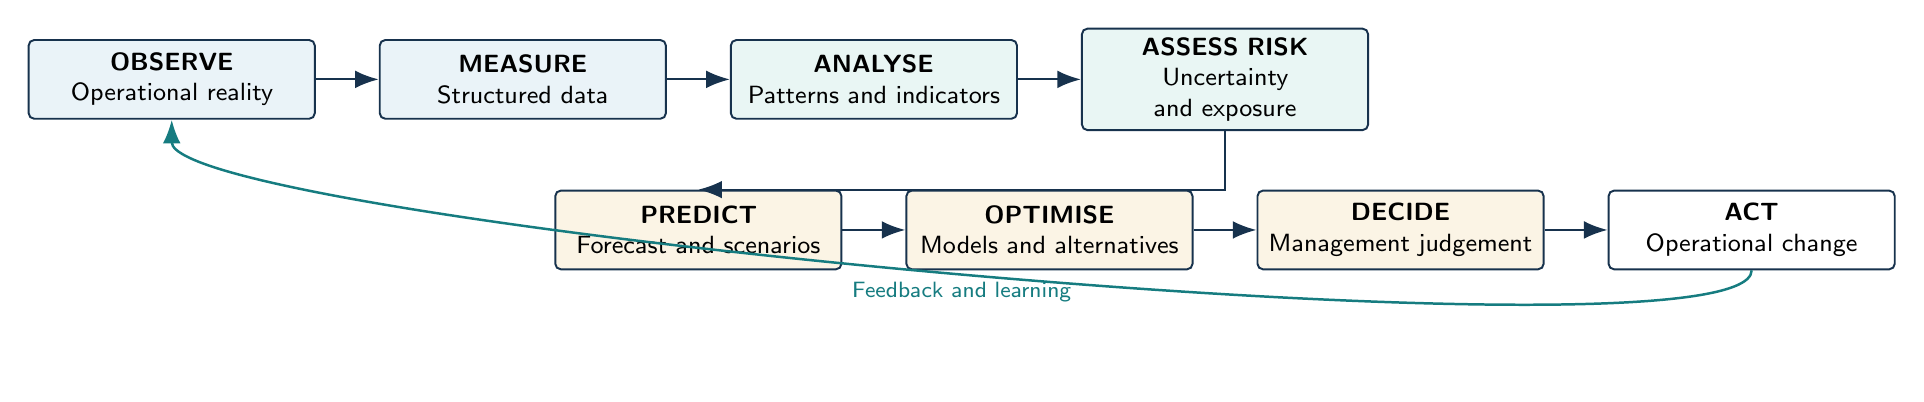
\begin{tikzpicture}[node distance=8mm]
\node[box,fill=lightblue] (observe) {\textbf{OBSERVE}\\Operational reality};
\node[box,right=of observe,fill=lightblue] (measure)
{\textbf{MEASURE}\\Structured data};
\node[box,right=of measure,fill=lightteal] (analyse)
{\textbf{ANALYSE}\\Patterns and indicators};
\node[box,right=of analyse,fill=lightteal] (risk)
{\textbf{ASSESS RISK}\\Uncertainty and exposure};

\node[box,below=14mm of $(measure)!0.5!(analyse)$,fill=lightgold]
(predict) {\textbf{PREDICT}\\Forecast and scenarios};
\node[box,right=of predict,fill=lightgold]
(optimise) {\textbf{OPTIMISE}\\Models and alternatives};
\node[box,right=of optimise,fill=lightgold]
(decide) {\textbf{DECIDE}\\Management judgement};
\node[box,right=of decide,fill=white]
(act) {\textbf{ACT}\\Operational change};

\draw[arrow] (observe)--(measure);
\draw[arrow] (measure)--(analyse);
\draw[arrow] (analyse)--(risk);
\draw[arrow] (risk.south) |- (predict.north);
\draw[arrow] (predict)--(optimise);
\draw[arrow] (optimise)--(decide);
\draw[arrow] (decide)--(act);
\draw[feedback] (act.south) .. controls +(0,-13mm) and +(0,-13mm) ..
  node[below,font=\sffamily\footnotesize\color{teal}]
  {Feedback and learning} (observe.south);
\end{tikzpicture}
\end{center}

This is the conceptual heart of Pharmacy V13.

\subsection{Observe}

The system captures evidence of what is occurring in the pharmacy.

\subsection{Measure}

Operational events are converted into reliable structured quantities,
positions, values, rates, and indicators.

\subsection{Analyse}

Patterns are identified across demand, inventory, purchasing, financial
activity, suppliers, and expiry.

\subsection{Assess risk}

The system identifies uncertainty and operational exposure rather than relying
only on averages.

\subsection{Predict}

Forecasting and simulation provide views of plausible future conditions.

\subsection{Optimise}

Decision models frame alternatives and trade-offs.

\subsection{Decide}

Management interprets the evidence in context and chooses an action.

\subsection{Act}

A decision changes purchasing, stock policy, planning, monitoring, or another
operational process.

\subsection{Feedback}

The consequences of action become new operational evidence, closing the loop.

% ============================================================
\section{Information, Knowledge, and Intelligence}

The architecture distinguishes three concepts that are often confused.

\begin{center}
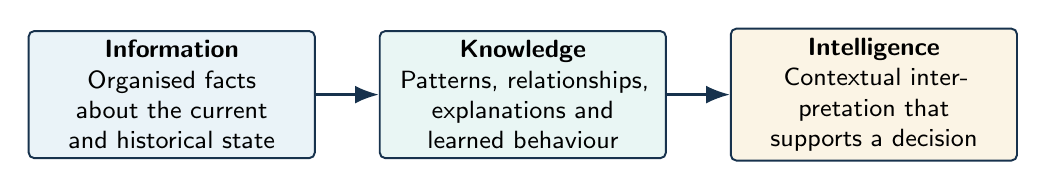
\begin{tikzpicture}[node distance=8mm]
\node[box,fill=lightblue] (info)
{\textbf{Information}\\
Organised facts about the current and historical state};

\node[box,right=of info,fill=lightteal] (knowledge)
{\textbf{Knowledge}\\
Patterns, relationships, explanations and learned behaviour};

\node[box,right=of knowledge,fill=lightgold] (intel)
{\textbf{Intelligence}\\
Contextual interpretation that supports a decision};

\draw[arrow] (info)--(knowledge);
\draw[arrow] (knowledge)--(intel);
\end{tikzpicture}
\end{center}

A dashboard that merely displays numbers provides information. A system that
identifies trends and relationships begins to provide knowledge. A system that
connects those findings to risk, context, alternatives, and management
questions provides decision intelligence.

% ============================================================
\section{Management Intelligence Cockpit}

The management dashboard should be designed around \textbf{attention and
decision flow}, rather than around the number of available reports.

A conceptual cockpit contains:

\begin{enumerate}
\item \textbf{Current state} --- What is happening now?
\item \textbf{Exceptions} --- What is outside expected behaviour?
\item \textbf{Risk} --- Where is exposure increasing?
\item \textbf{Prediction} --- What is likely to happen next?
\item \textbf{Priority} --- What deserves attention first?
\item \textbf{Explanation} --- Why is this being highlighted?
\item \textbf{Action context} --- What options are available?
\item \textbf{Feedback} --- What happened after the action?
\end{enumerate}

The dashboard should therefore function as a \textbf{management awareness
interface}, not simply a collection of charts.

% ============================================================
\section{Governance and Model Transparency}

Decision intelligence must remain auditable.

Each significant analytical output should, conceptually, be associated with:

\begin{itemize}
\item the data period used;
\item the relevant data sources;
\item the model or method used;
\item key assumptions;
\item data freshness;
\item uncertainty or confidence information where appropriate;
\item the policy thresholds or parameters applied;
\item the resulting recommendation or alert;
\item the human decision and, where appropriate, the reason for overriding it.
\end{itemize}

This creates a chain:

\[
\text{Evidence}
\rightarrow
\text{Model}
\rightarrow
\text{Interpretation}
\rightarrow
\text{Recommendation}
\rightarrow
\text{Decision}
\rightarrow
\text{Outcome}.
\]

Such traceability is essential when the system evolves from reporting toward
AI-assisted decision support.

% ============================================================
\section{Performance and Continuous Learning}

A mature V13 architecture should measure not only pharmacy operations but also
the performance of its analytical intelligence.

Examples include:

\begin{center}
\renewcommand{\arraystretch}{1.35}
\begin{tabularx}{\textwidth}{>{\bfseries}p{36mm} X}
\toprule
Performance area & Example management concern \\
\midrule
Service and availability & Are important items available when required? \\
Inventory efficiency & Is capital being held efficiently? \\
Expiry exposure & Is vulnerable inventory being identified early? \\
Supplier performance & Are lead times and purchasing reliability acceptable? \\
Forecast quality & How well do forecasts correspond to subsequent demand? \\
Decision effectiveness & Did actions reduce the identified risk or improve the target? \\
Data quality & Can management trust the evidence on which intelligence is based? \\
\bottomrule
\end{tabularx}
\end{center}

This enables a second feedback loop:

\[
\text{Operational feedback}
+
\text{Model performance}
\rightarrow
\text{Continuous improvement}.
\]

Thus V13 can evolve from a static information system toward a learning
management platform.

% ============================================================
\section{Decision Support, Not Automated Management}

A central architectural boundary is the distinction between \textbf{decision
support} and \textbf{decision authority}.

The system can:

\begin{itemize}
\item identify a shortage risk;
\item forecast demand;
\item estimate safety stock;
\item highlight expiry exposure;
\item simulate possible outcomes;
\item rank management priorities;
\item explain analytical findings;
\item suggest options.
\end{itemize}

Management remains responsible for:

\begin{itemize}
\item validating context;
\item considering operational constraints;
\item applying professional and institutional judgement;
\item authorising action;
\item evaluating consequences.
\end{itemize}

\begin{principle}[Human-in-the-loop architecture]
\centering
\large
\textbf{The system supplies evidence, analysis, prediction and options.\\
Management supplies context, judgement, authority and accountability.}
\end{principle}

% ============================================================
\section{What Pharmacy V13 Is}

Pharmacy V13 can therefore be defined as:

\begin{keyidea}[System Definition]
\textbf{Pharmacy V13 is an integrated management intelligence and
decision-support architecture that transforms pharmacy operational evidence
into structured information, analytical knowledge, risk-aware predictions and
AI-assisted management insight, enabling accountable decisions and continuous
feedback between management action and operational reality.}
\end{keyidea}

Its conceptual architecture is not defined by the number of screens, records,
medicines, tables, or transactions. Those are implementation details.

Its defining characteristic is the transformation of operational reality into
decision intelligence.

% ============================================================
\section{What Belongs in the System Reference}

A conceptual reference should describe the stable architecture of the system.

\subsection*{Appropriate content}

\begin{itemize}
\item system purpose and philosophy;
\item operational-to-management information flow;
\item analytical architecture;
\item decision models and their management questions;
\item AI integration principles;
\item management hierarchy;
\item feedback and learning architecture;
\item governance and transparency;
\item conceptual KPIs and performance dimensions.
\end{itemize}

\subsection*{Operational material that belongs elsewhere}

\begin{itemize}
\item current inventory lists;
\item individual medicine names;
\item current transaction records;
\item temporary test data;
\item individual supplier records;
\item current database contents;
\item transient operational screenshots;
\item deployment logs and implementation diagnostics.
\end{itemize}

Those materials are valuable operational artifacts, but they should not define
the conceptual identity of V13.

% ============================================================
\section{Model Summary}

\begin{center}
\renewcommand{\arraystretch}{1.5}
\begin{longtable}{>{\bfseries}p{33mm} p{45mm} p{62mm}}
\toprule
Model & Question & Management meaning \\
\midrule
Forecasting &
What demand should we expect? &
Provides an evidence-based expectation of future consumption. \\
ROP &
When should replenishment be triggered? &
Connects expected lead-time demand with a replenishment threshold. \\
Safety Stock &
How much uncertainty protection is needed? &
Provides a buffer against demand and supply variability. \\
EOQ &
What order quantity balances costs? &
Frames the economic trade-off between ordering and holding. \\
ABC &
Where should management attention be concentrated? &
Prioritises inventory according to value or selected importance criteria. \\
Expiry Risk &
Where is stock vulnerable because of remaining shelf life? &
Compares expected consumption with remaining time to expiry. \\
Monte Carlo &
What could happen under uncertainty? &
Produces a distribution of possible outcomes and associated probabilities. \\
AI Integrated View &
What deserves attention and why? &
Synthesises evidence and model outputs into an interpretable management view. \\
\bottomrule
\end{longtable}
\end{center}

% ============================================================
\section{Conclusion}

Pharmacy V13 should be understood as a \textbf{closed-loop management
intelligence system}.

Its fundamental progression is:

\[
\boxed{
\text{Operational Reality}
\rightarrow
\text{Data}
\rightarrow
\text{Information}
\rightarrow
\text{Knowledge}
\rightarrow
\text{Intelligence}
\rightarrow
\text{Decision}
\rightarrow
\text{Action}
\rightarrow
\text{Feedback}
}
\]

The operational system provides evidence. The database preserves memory. The
analytical layer provides reasoning. Forecasting and simulation expose possible
futures. Risk models identify vulnerability. Optimisation models frame
trade-offs. AI integrates signals and helps communicate their meaning. The
management layer converts this intelligence into accountable action.

The resulting architecture can be summarised in one sentence:

\begin{center}
\Large
\textbf{\color{navy}
Transaction $\rightarrow$ Information $\rightarrow$ Analysis
$\rightarrow$ Intelligence $\rightarrow$ Decision $\rightarrow$ Action.}
\end{center}

That is the conceptual identity of Pharmacy V13.

\vfill

\begin{center}
\sffamily\small
\textit{Pharmacy V13 --- Management Intelligence and Decision-Support Architecture}\\
Conceptual System Reference \quad | \quad Version 1.0 \quad | \quad 2026
\end{center}

\end{document}
